\section{Validation}\label{appendix:prediction_accuracy}
\subsection{Prediction Accuracy}
\begin{table}[ht]
    \centering
    \resizebox{\columnwidth}{!}                         \\ \cline{3-8} 
    \multicolumn{2}{|l}{}                                                           & \multicolumn{3}{c|}{$d_{1}$} & \multicolumn{3}{c|}{$d_{2}$}                   \\ \hline
    \multicolumn{2}{|c|}{Dataset size} &
        \multicolumn{1}{l|}{1400} &
        \multicolumn{1}{l|}{5120} &
        \multicolumn{1}{l|}{10240} &
        \multicolumn{1}{l|}{1400} &
        \multicolumn{1}{l|}{5120} &
        10240 \\ \hline
    \multicolumn{1}{|c|}{\multirow{3}{*}{Bin resolution}} & \multicolumn{1}{l|}{5}  & 92.73  & 92.84  & 93.13 & 96.36 & 96.76                     & 96.73 \\ \cline{2-2}
    \multicolumn{1}{|c|}{}                                & \multicolumn{1}{l|}{7}  & 93.74  & 94.08  & 94.79 & 96.98 & 96.79                     & 97.00 \\ \cline{2-2}
    \multicolumn{1}{|c|}{}                                & \multicolumn{1}{l|}{10} & 89.37  & 91.20  & 90.86 & 88.25 & \multicolumn{1}{r}{89.75} & 89.40 \\ \hline
    \end{tabular}%
    }
    \caption{\small A table displaying the average accuracy of predictions for $d_{1}$ and $d_{2}$ errors while investigating variations in both (i) the size of the dataset and (ii) the resolution of bins.}
    \label{tab:prediction_accuracy}
\end{table}

\newpage
\subsection{K-Fold Cross Validation}

\begin{figure*}[h!]
    \centering
    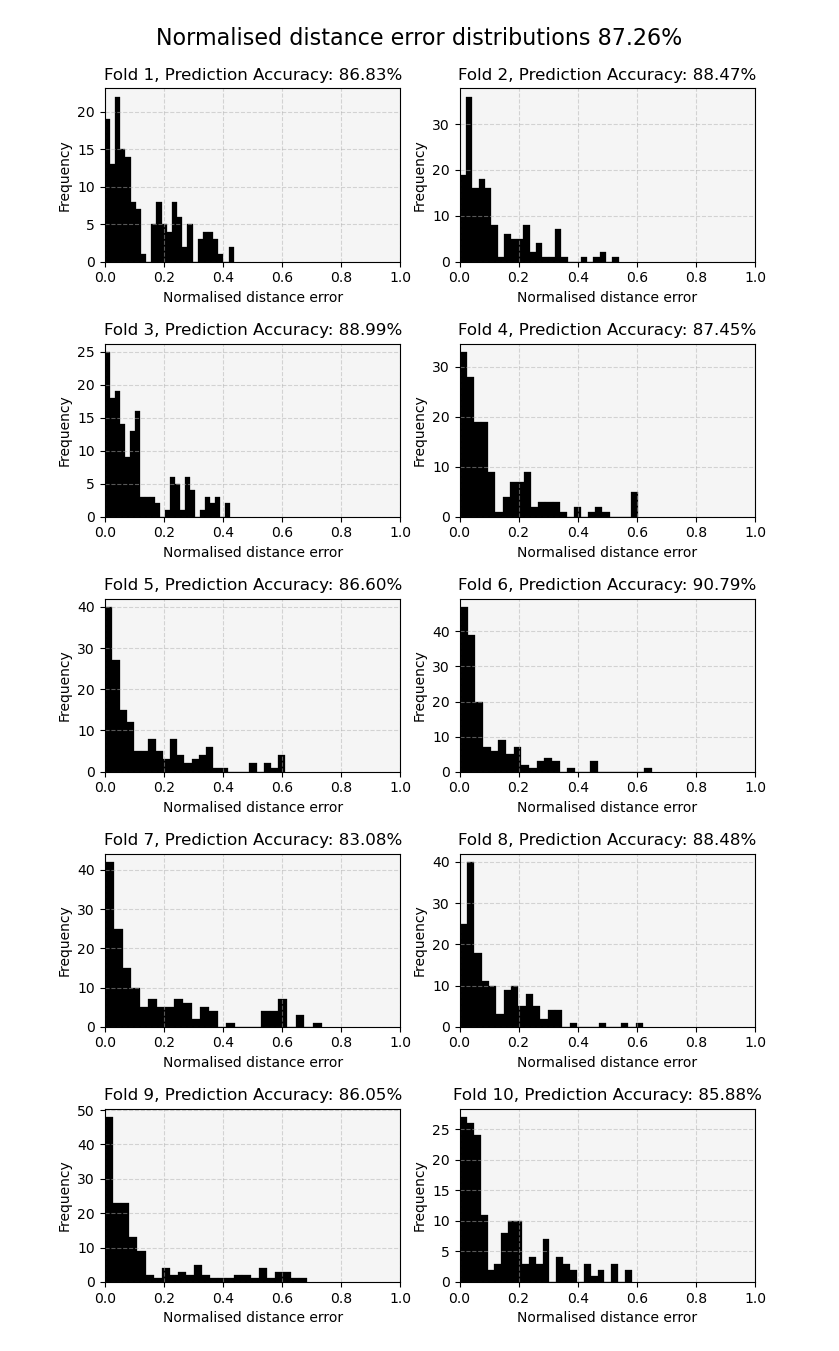
\includegraphics[width=0.65\textwidth]{figures/validation_plots/TE/k-fold_two_outputs.png}
    \caption{\small Normalised probability histograms with prediction accuracy values for each fold is shown for $d_{1}$ bin configuration: inputs (7) outputs (5), dataset size = 10240.}~\label{fig:k-foldhistogramsTE}
\end{figure*}

\newpage
\section{Bayesian Reverse Inference}

% 2 outputs: 

% \begin{figure*}[ht]
%     \centering
%     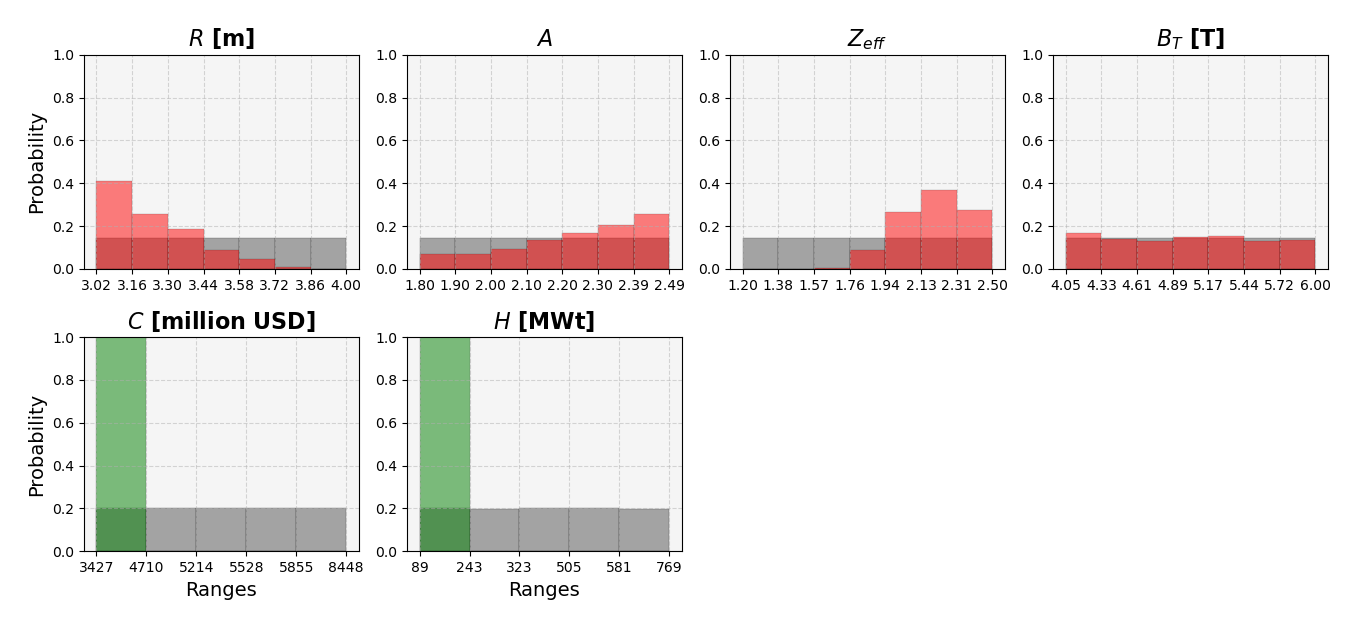
\includegraphics[width=0.6\textwidth]{figures/TE_results/march_data/config(57)_2outputs_1.png}
%     \caption{Resulting posterior distributions depicted in red (variables: Major Radius $R$, Aspect Ratio $A$, Effective Ion Charge $Z_{\text{eff}}$, Toroidal Field on Plasma $B_{\text{T}}$) for reverse
%     inference on the selected green bins (High Grade Wasteheat $H$, Capital Cost $C$) after updating the marginal prior beliefs (grey).}~\label{fig:config(57)_2outputs_1}
% \end{figure*}

% \begin{figure*}[ht]
%     \centering
%     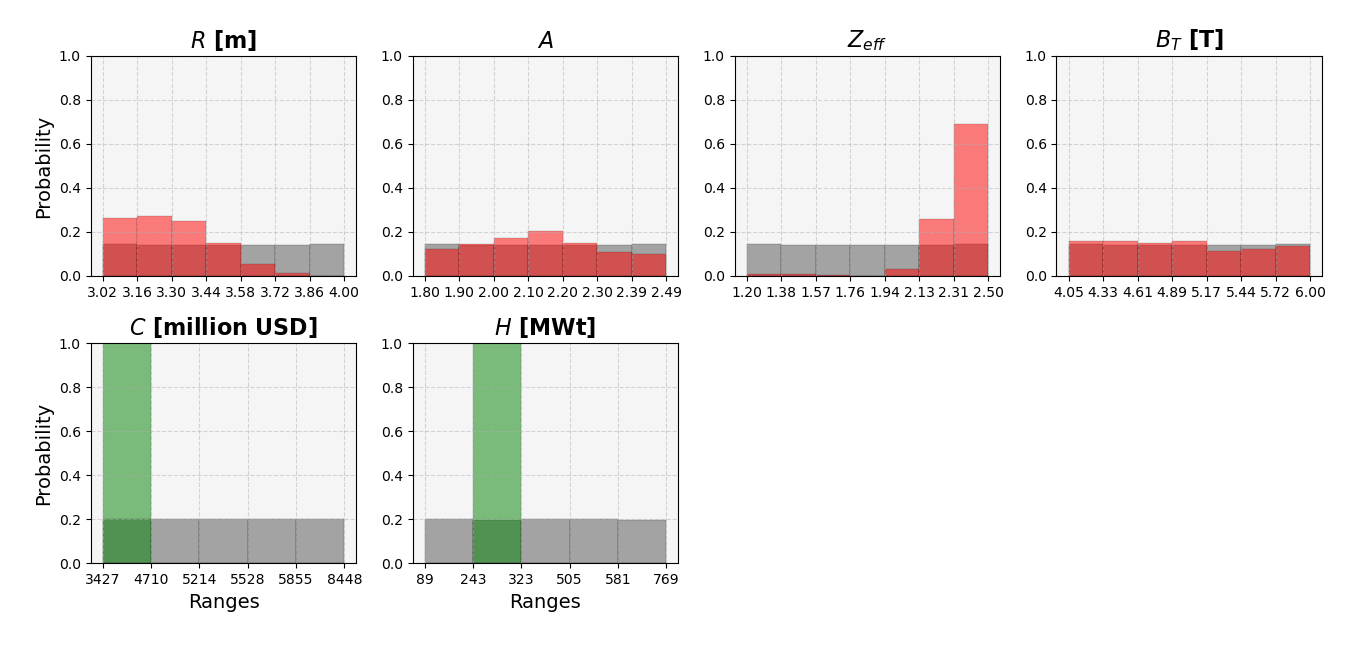
\includegraphics[width=0.6\textwidth]{figures/TE_results/march_data/config(57)_2outputs_2.png}
%     \caption{Resulting posterior distributions depicted in red (variables: Major Radius $R$, Aspect Ratio $A$, Effective Ion Charge $Z_{\text{eff}}$, Toroidal Field on Plasma $B_{\text{T}}$) for reverse
%     inference on the selected green bins (High Grade Wasteheat $H$, Capital Cost $C$) after updating the marginal prior beliefs (grey).}~\label{fig:config(57)_2outputs_2}
% \end{figure*}

% \begin{figure*}[ht]
%     \centering
%     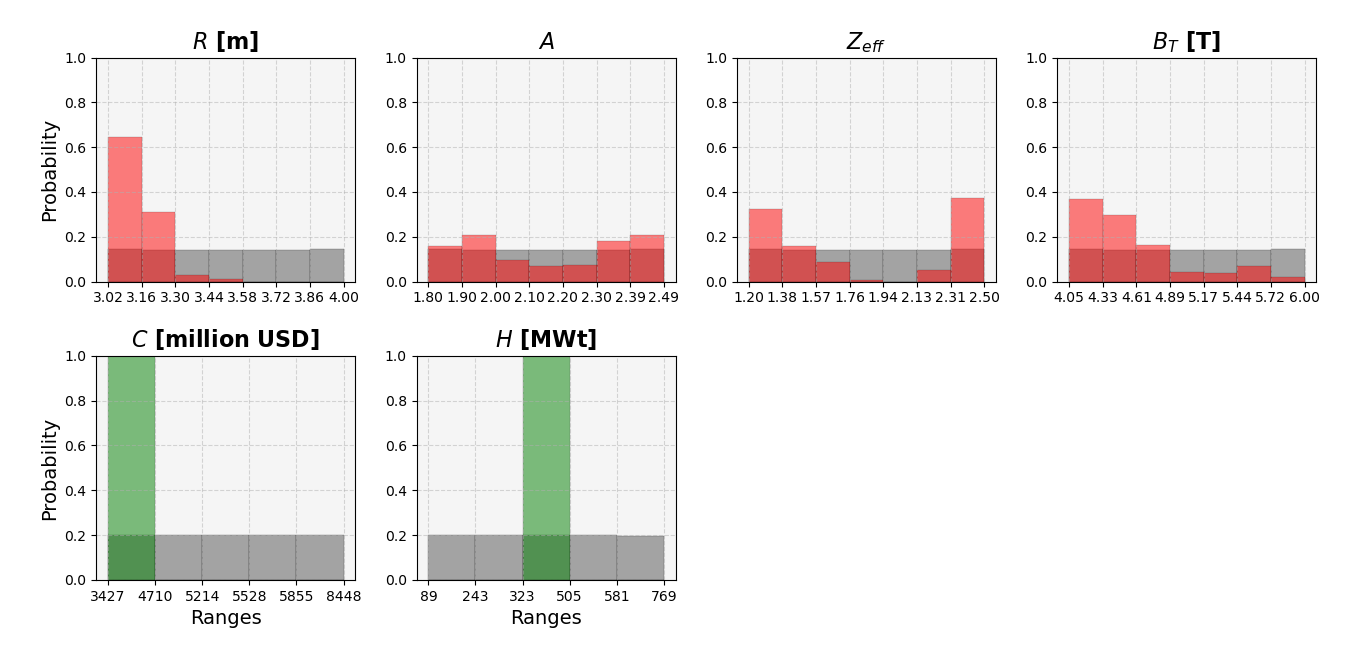
\includegraphics[width=0.6\textwidth]{figures/TE_results/march_data/config(57)_2outputs_3.png}
%     \caption{Resulting posterior distributions depicted in red (variables: Major Radius $R$, Aspect Ratio $A$, Effective Ion Charge $Z_{\text{eff}}$, Toroidal Field on Plasma $B_{\text{T}}$) for reverse
%     inference on the selected green bins (High Grade Wasteheat $H$, Capital Cost $C$) after updating the marginal prior beliefs (grey).}~\label{fig:config(57)_2outputs_3}
% \end{figure*}

% \begin{figure*}[ht]
%     \centering
%     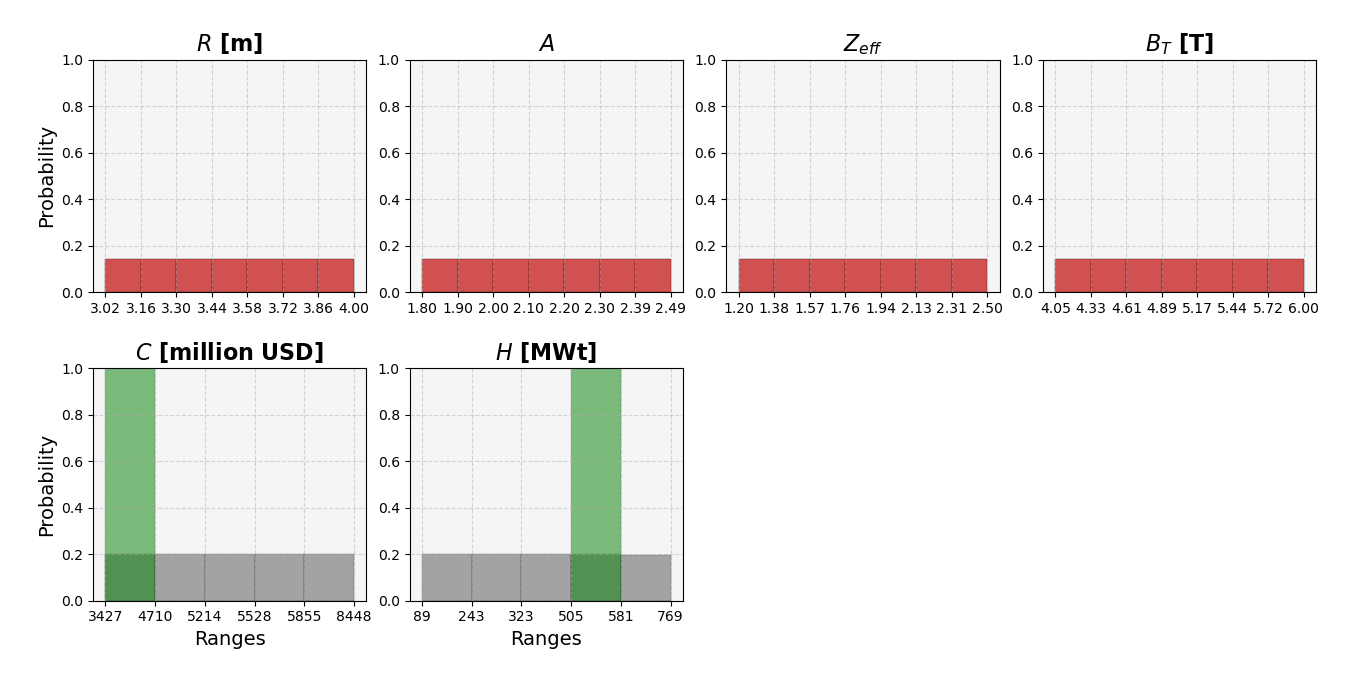
\includegraphics[width=0.6\textwidth]{figures/TE_results/march_data/config(57)_2outputs_4.png}
%     \caption{Resulting posterior distributions depicted in red (variables: Major Radius $R$, Aspect Ratio $A$, Effective Ion Charge $Z_{\text{eff}}$, Toroidal Field on Plasma $B_{\text{T}}$) for reverse
%     inference on the selected green bins (High Grade Wasteheat $H$, Capital Cost $C$) after updating the marginal prior beliefs (grey).}~\label{fig:config(57)_2outputs_4}
% \end{figure*}

% \begin{figure*}[ht]
%     \centering
%     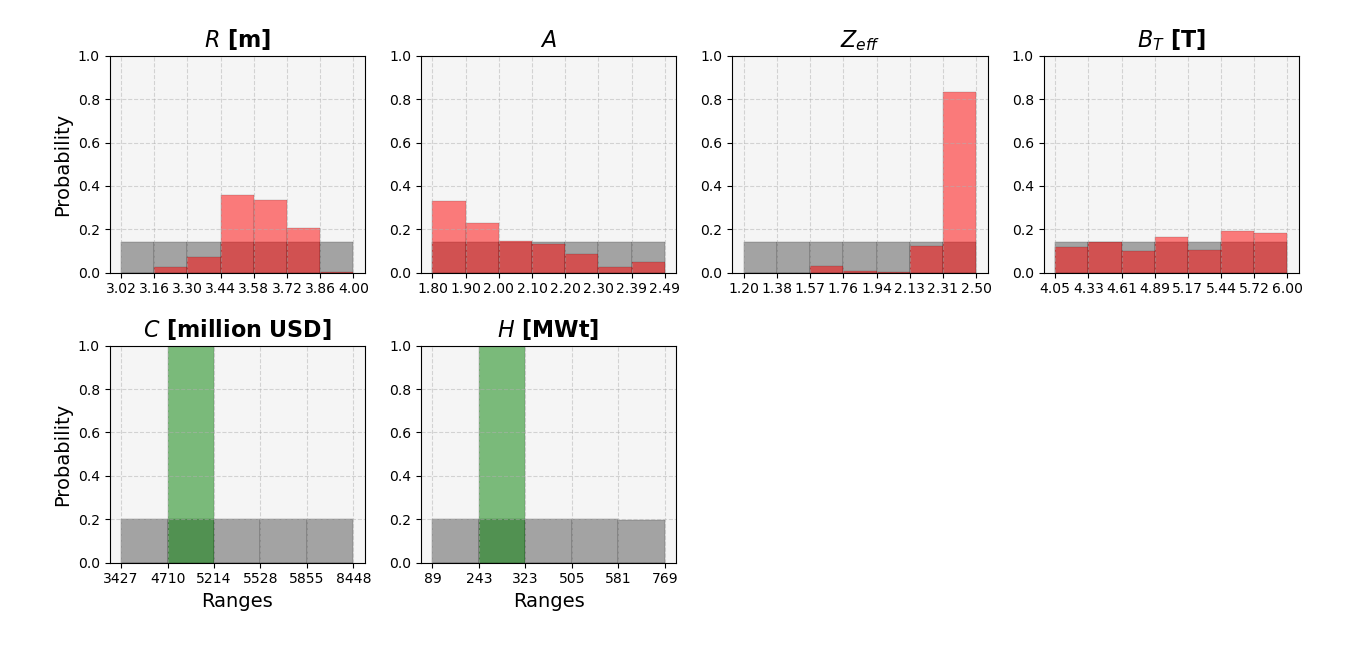
\includegraphics[width=0.6\textwidth]{figures/TE_results/march_data/config(57)_2outputs_6.png}
%     \caption{Resulting posterior distributions depicted in red (variables: Major Radius $R$, Aspect Ratio $A$, Effective Ion Charge $Z_{\text{eff}}$, Toroidal Field on Plasma $B_{\text{T}}$) for reverse
%     inference on the selected green bins (High Grade Wasteheat $H$, Capital Cost $C$) after updating the marginal prior beliefs (grey).}~\label{fig:config(57)_2outputs_6}
% \end{figure*}

% \begin{figure*}[ht]
%     \centering
%     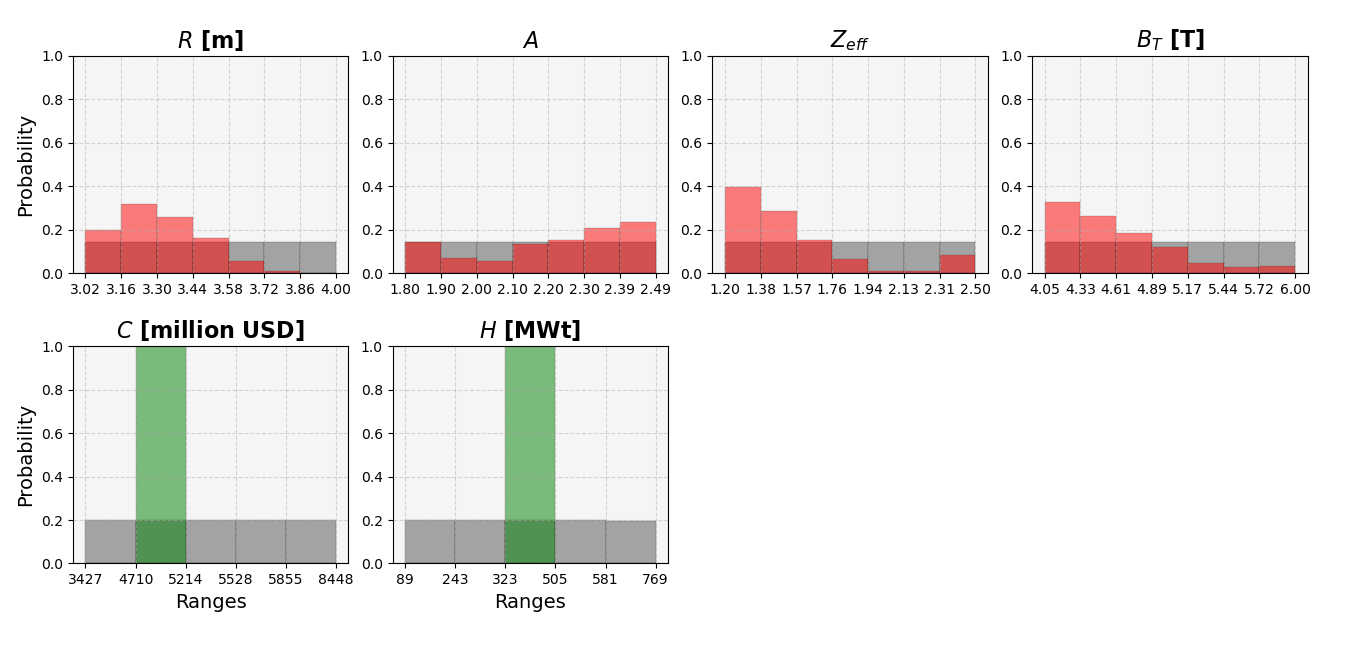
\includegraphics[width=0.6\textwidth]{figures/TE_results/march_data/config(57)_2outputs_7.png}
%     \caption{Resulting posterior distributions depicted in red (variables: Major Radius $R$, Aspect Ratio $A$, Effective Ion Charge $Z_{\text{eff}}$, Toroidal Field on Plasma $B_{\text{T}}$) for reverse
%     inference on the selected green bins (High Grade Wasteheat $H$, Capital Cost $C$) after updating the marginal prior beliefs (grey).}\label{fig:config(57)_2outputs_7}
% \end{figure*}

% \begin{figure*}[ht]
%     \centering
%     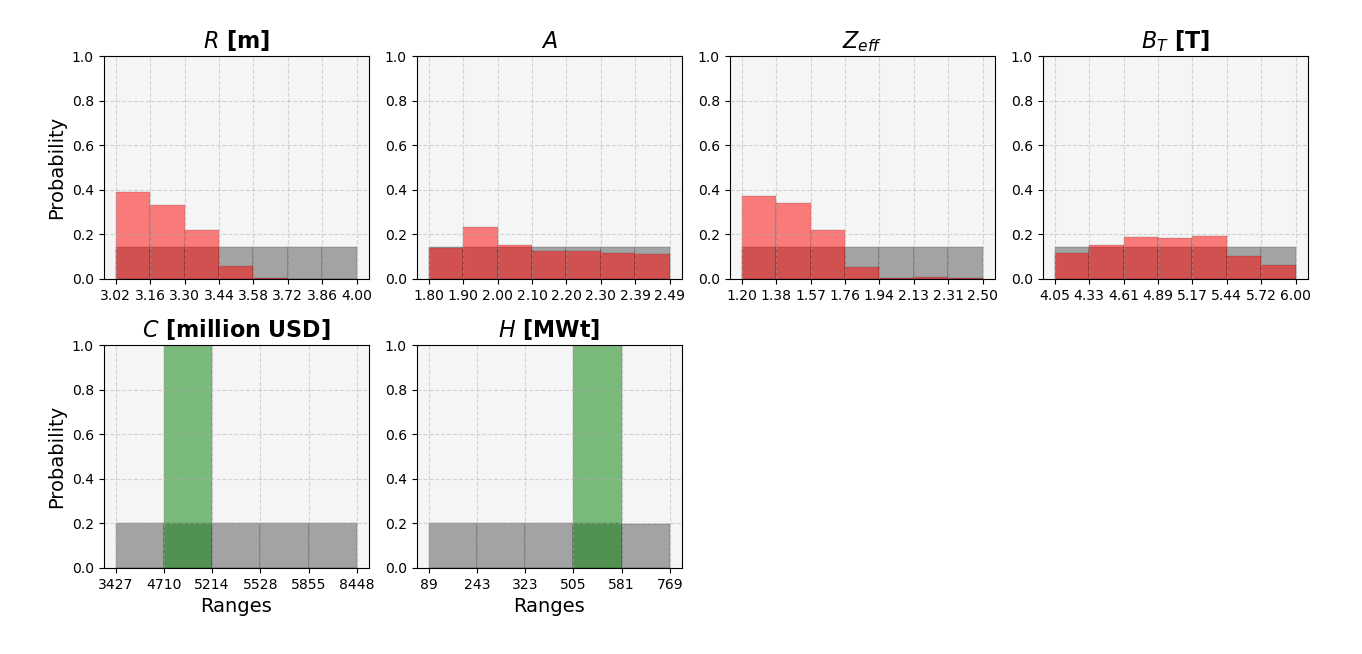
\includegraphics[width=0.6\textwidth]{figures/TE_results/march_data/config(57)_2outputs_8.png}
%     \caption{Resulting posterior distributions depicted in red (variables: Major Radius $R$, Aspect Ratio $A$, Effective Ion Charge $Z_{\text{eff}}$, Toroidal Field on Plasma $B_{\text{T}}$) for reverse
%     inference on the selected green bins (High Grade Wasteheat $H$, Capital Cost $C$) after updating the marginal prior beliefs (grey).}~\label{fig:config(57)_2outputs_8}
% \end{figure*}

% \begin{figure*}[ht]
%     \centering
%     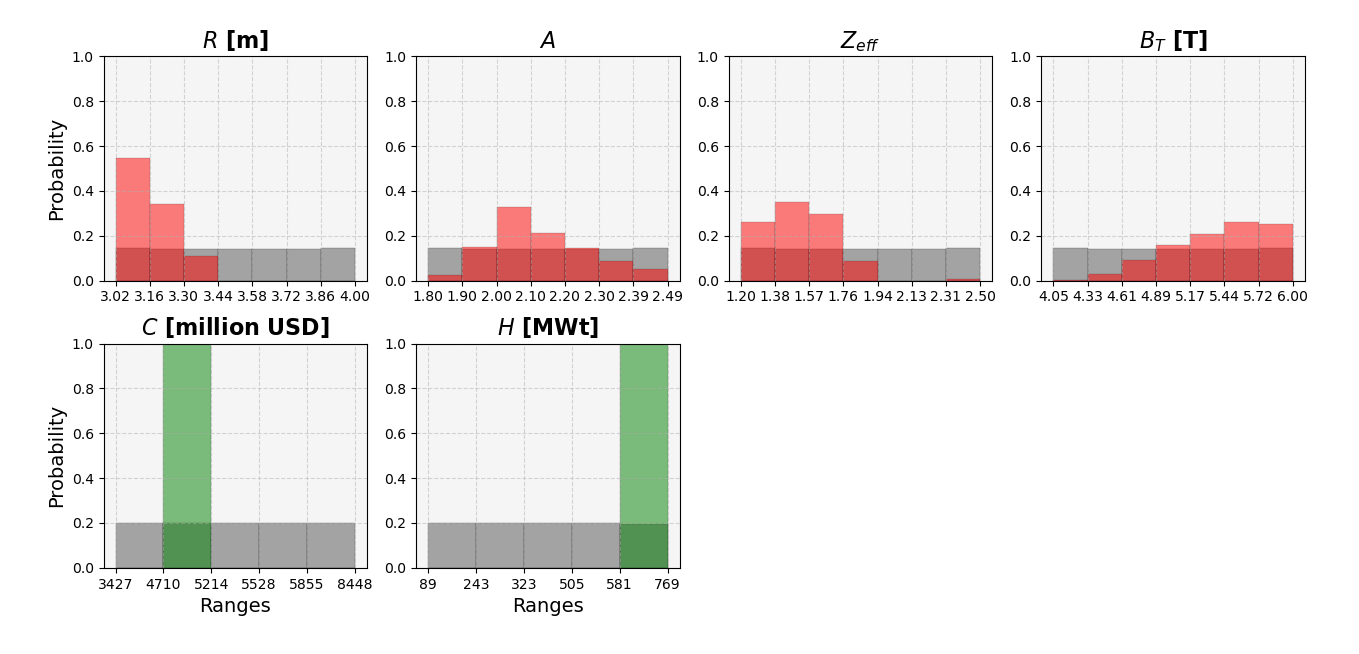
\includegraphics[width=0.6\textwidth]{figures/TE_results/march_data/config(57)_2outputs_9.png}
%     \caption{Resulting posterior distributions depicted in red (variables: Major Radius $R$, Aspect Ratio $A$, Effective Ion Charge $Z_{\text{eff}}$, Toroidal Field on Plasma $B_{\text{T}}$) for reverse
%     inference on the selected green bins (High Grade Wasteheat $H$, Capital Cost $C$) after updating the marginal prior beliefs (grey).}~\label{fig:config(57)_2outputs_9}
% \end{figure*}

% \begin{figure*}[ht]
%     \centering
%     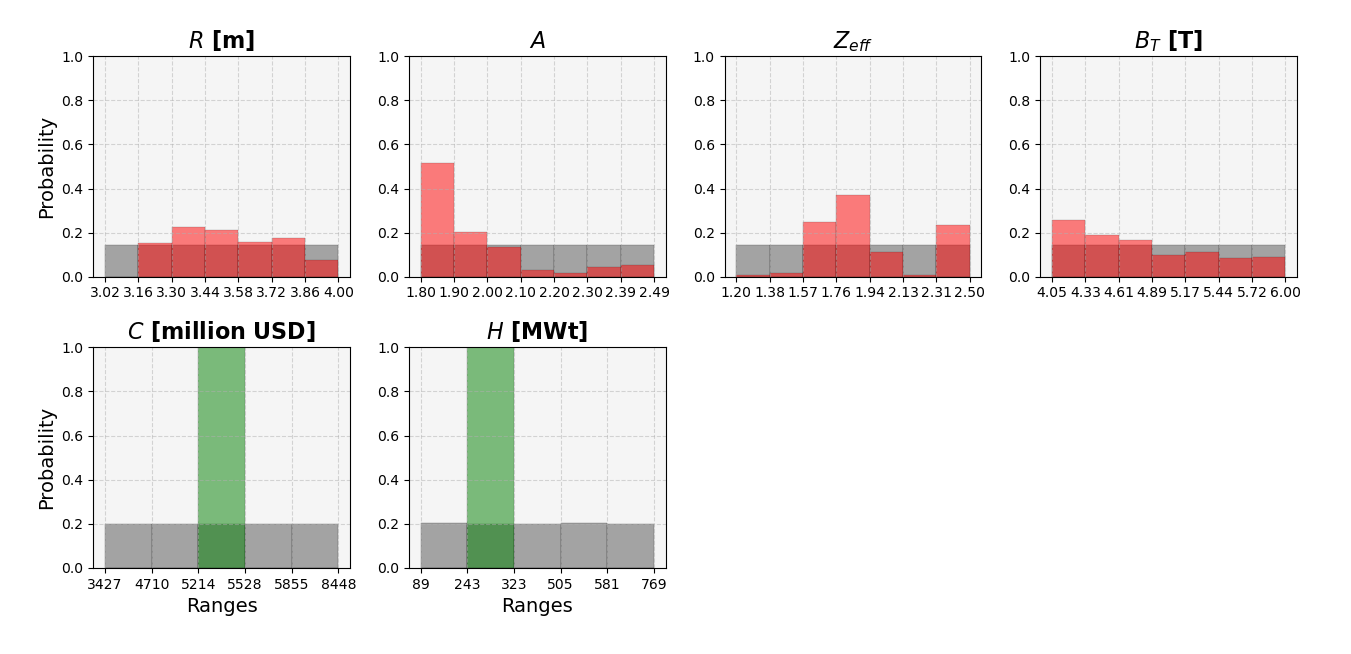
\includegraphics[width=0.6\textwidth]{figures/TE_results/march_data/config(57)_2outputs_10.png}
%     \caption{Resulting posterior distributions depicted in red (variables: Major Radius $R$, Aspect Ratio $A$, Effective Ion Charge $Z_{\text{eff}}$, Toroidal Field on Plasma $B_{\text{T}}$) for reverse
%     inference on the selected green bins (High Grade Wasteheat $H$, Capital Cost $C$) after updating the marginal prior beliefs (grey).}~\label{fig:config(57)_2outputs_10}
% \end{figure*}

% \begin{figure*}[ht]
%     \centering
%     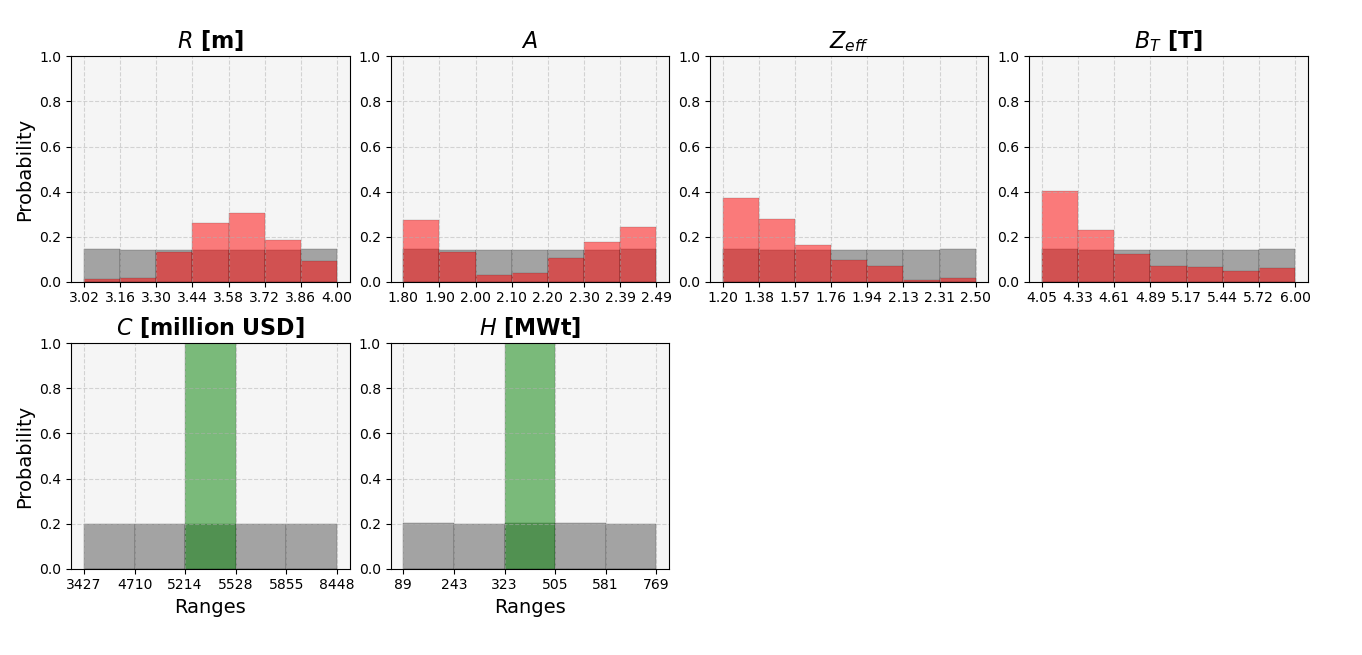
\includegraphics[width=0.6\textwidth]{figures/TE_results/march_data/config(57)_2outputs_11.png}
%     \caption{Resulting posterior distributions depicted in red (variables: Major Radius $R$, Aspect Ratio $A$, Effective Ion Charge $Z_{\text{eff}}$, Toroidal Field on Plasma $B_{\text{T}}$) for reverse
%     inference on the selected green bins (High Grade Wasteheat $H$, Capital Cost $C$) after updating the marginal prior beliefs (grey).}~\label{fig:config(57)_2outputs_11}
% \end{figure*}

% \begin{figure*}[ht]
%     \centering
%     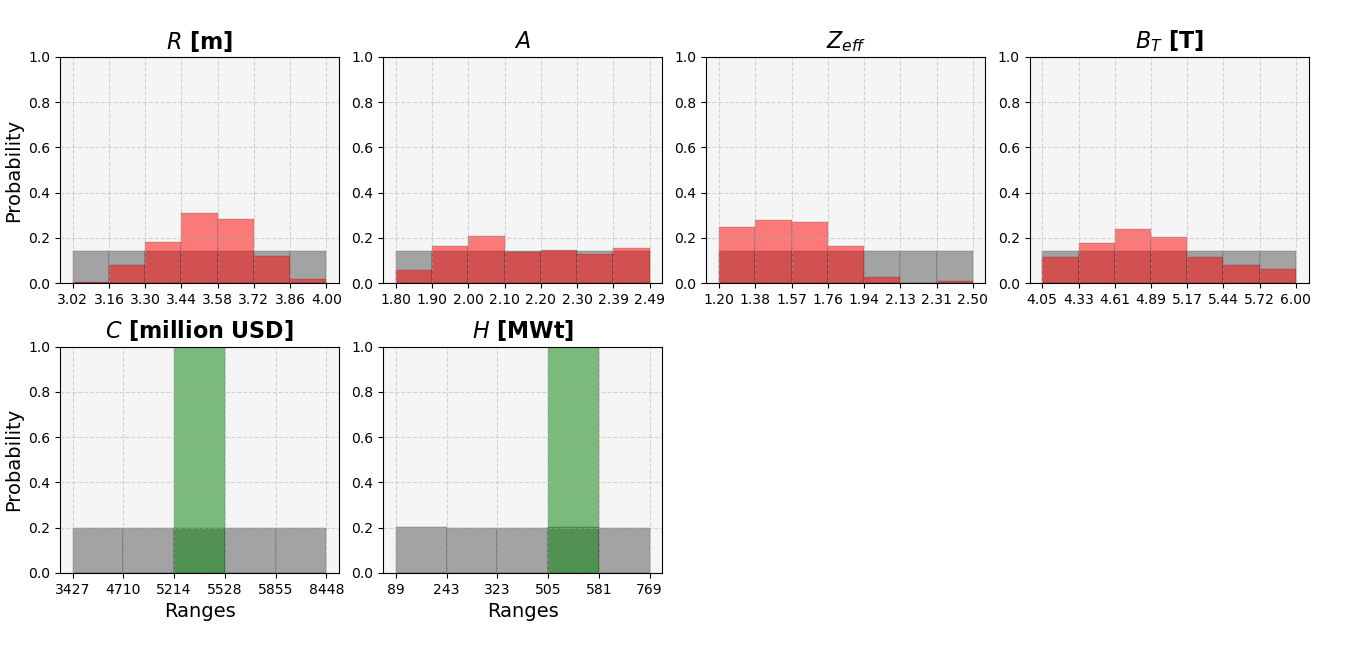
\includegraphics[width=0.6\textwidth]{figures/TE_results/march_data/config(57)_2outputs_12.png}
%     \caption{Resulting posterior distributions depicted in red (variables: Major Radius $R$, Aspect Ratio $A$, Effective Ion Charge $Z_{\text{eff}}$, Toroidal Field on Plasma $B_{\text{T}}$) for reverse
%     inference on the selected green bins (High Grade Wasteheat $H$, Capital Cost $C$) after updating the marginal prior beliefs (grey).}~\label{fig:config(57)_2outputs_12}
% \end{figure*}

% \begin{figure*}[ht]
%     \centering
%     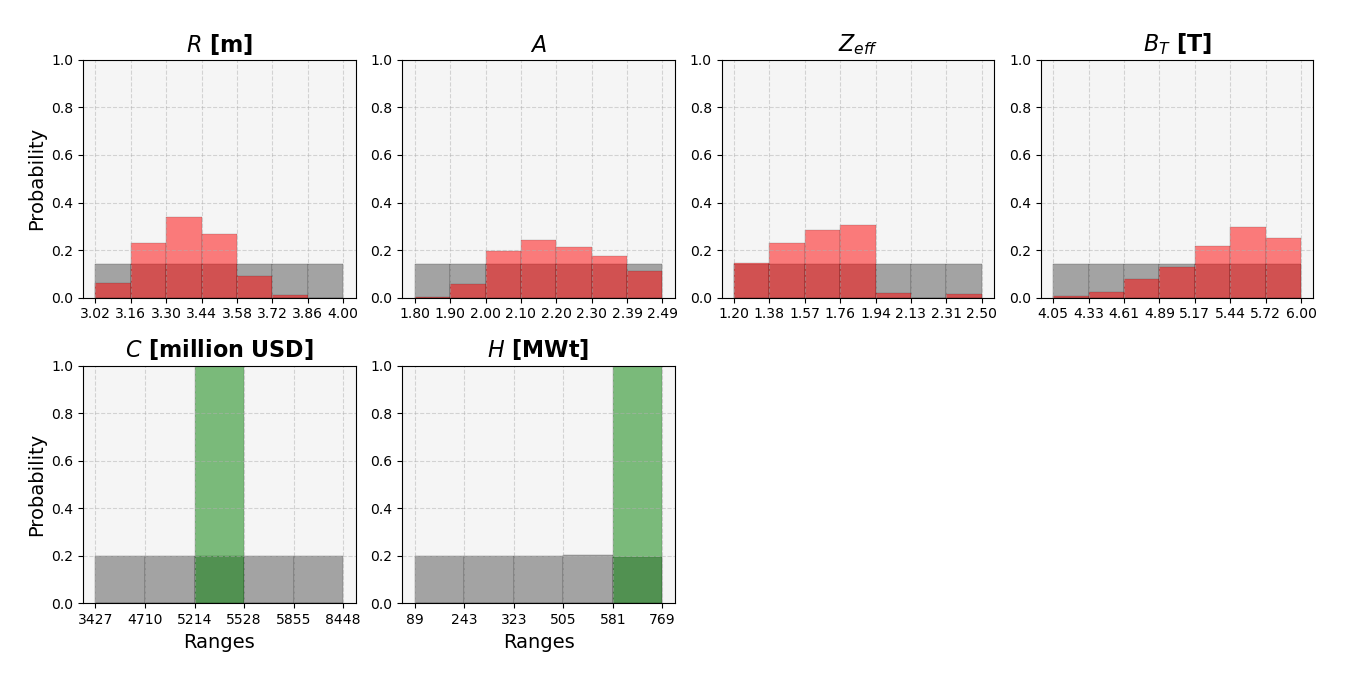
\includegraphics[width=0.6\textwidth]{figures/TE_results/march_data/config(57)_2outputs_125.png}
%     \caption{Resulting posterior distributions depicted in red (variables: Major Radius $R$, Aspect Ratio $A$, Effective Ion Charge $Z_{\text{eff}}$, Toroidal Field on Plasma $B_{\text{T}}$) for reverse
%     inference on the selected green bins (High Grade Wasteheat $H$, Capital Cost $C$) after updating the marginal prior beliefs (grey).}~\label{fig:config(57)_2outputs_125}
% \end{figure*}

% \begin{figure*}[ht]
%     \centering
%     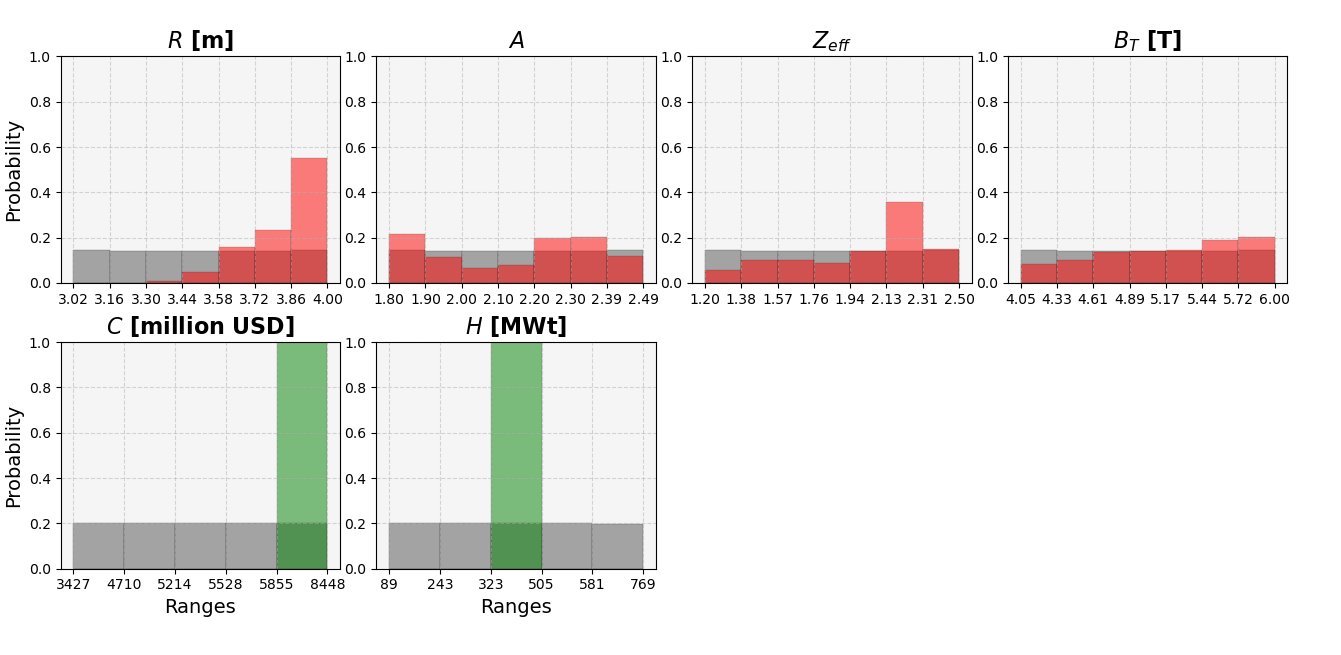
\includegraphics[width=0.6\textwidth]{figures/TE_results/march_data/config(57)_2outputs_16.png}
%     \caption{Resulting posterior distributions depicted in red (variables: Major Radius $R$, Aspect Ratio $A$, Effective Ion Charge $Z_{\text{eff}}$, Toroidal Field on Plasma $B_{\text{T}}$) for reverse
%     inference on the selected green bins (High Grade Wasteheat $H$, Capital Cost $C$) after updating the marginal prior beliefs (grey).}~\label{fig:config(57)_2outputs_16}
% \end{figure*}

% \begin{figure*}[ht]
%     \centering
%     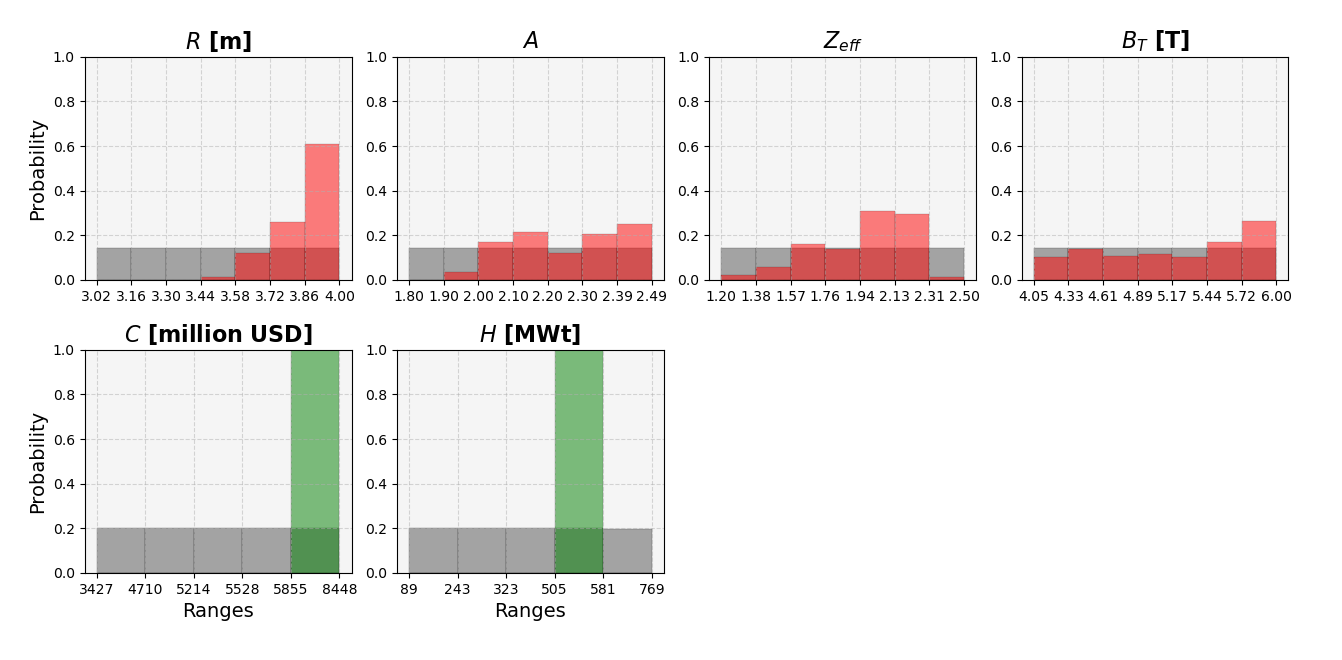
\includegraphics[width=0.6\textwidth]{figures/TE_results/march_data/config(57)_2outputs_17.png}
%     \caption{Resulting posterior distributions depicted in red (variables: Major Radius $R$, Aspect Ratio $A$, Effective Ion Charge $Z_{\text{eff}}$, Toroidal Field on Plasma $B_{\text{T}}$) for reverse
%     inference on the selected green bins (High Grade Wasteheat $H$, Capital Cost $C$) after updating the marginal prior beliefs (grey).}~\label{fig:config(57)_2outputs_17}
% \end{figure*}

% \begin{figure*}[ht]
%     \centering
%     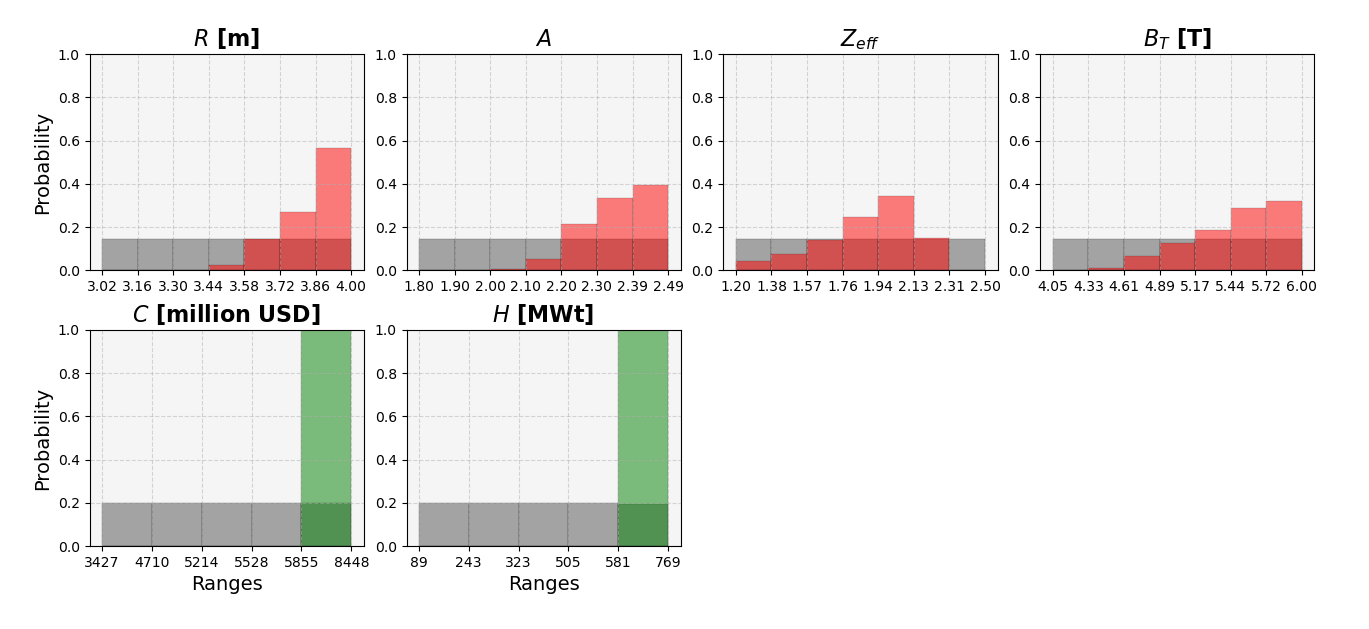
\includegraphics[width=0.6\textwidth]{figures/TE_results/march_data/config(57)_2outputs_18.png}
%     \caption{Resulting posterior distributions depicted in red (variables: Major Radius $R$, Aspect Ratio $A$, Effective Ion Charge $Z_{\text{eff}}$, Toroidal Field on Plasma $B_{\text{T}}$) for reverse
%     inference on the selected green bins (High Grade Wasteheat $H$, Capital Cost $C$) after updating the marginal prior beliefs (grey).}~\label{fig:config(57)_2outputs_18}
% \end{figure*}

\begin{figure*}[ht]
    \centering
    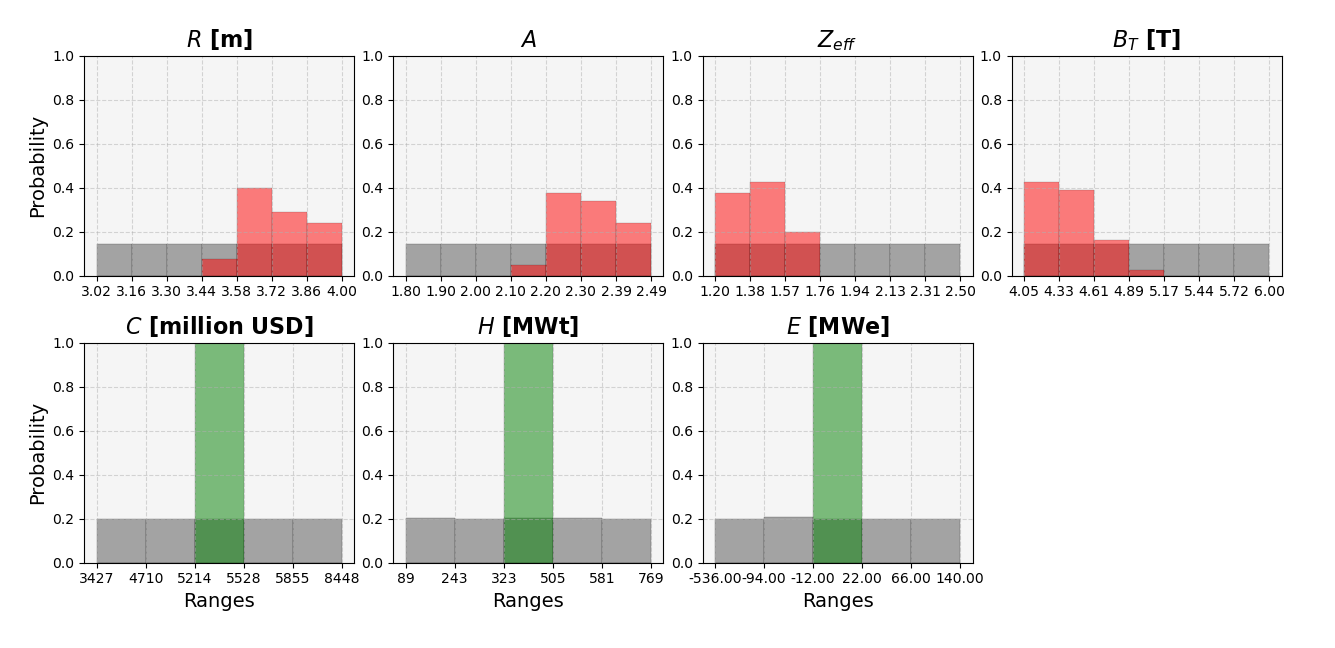
\includegraphics[width=0.6\textwidth]{figures/TE_results/march_data/config(57)_3outputs_V2_1.png}
    \caption{Resulting posterior distributions depicted in red (variables: Major Radius $R$, Aspect Ratio $A$, Effective Ion Charge $Z_{\text{eff}}$, Toroidal Field on Plasma $B_{\text{T}}$) for reverse
    inference on the selected green bins (High Grade Wasteheat $H$, Net Electrical Output $E$, and  Capital Cost $C$) after updating the marginal prior beliefs (grey).}~\label{fig:config(57)_3outputs_V2_1}
\end{figure*}

\begin{figure*}[ht]
    \centering
    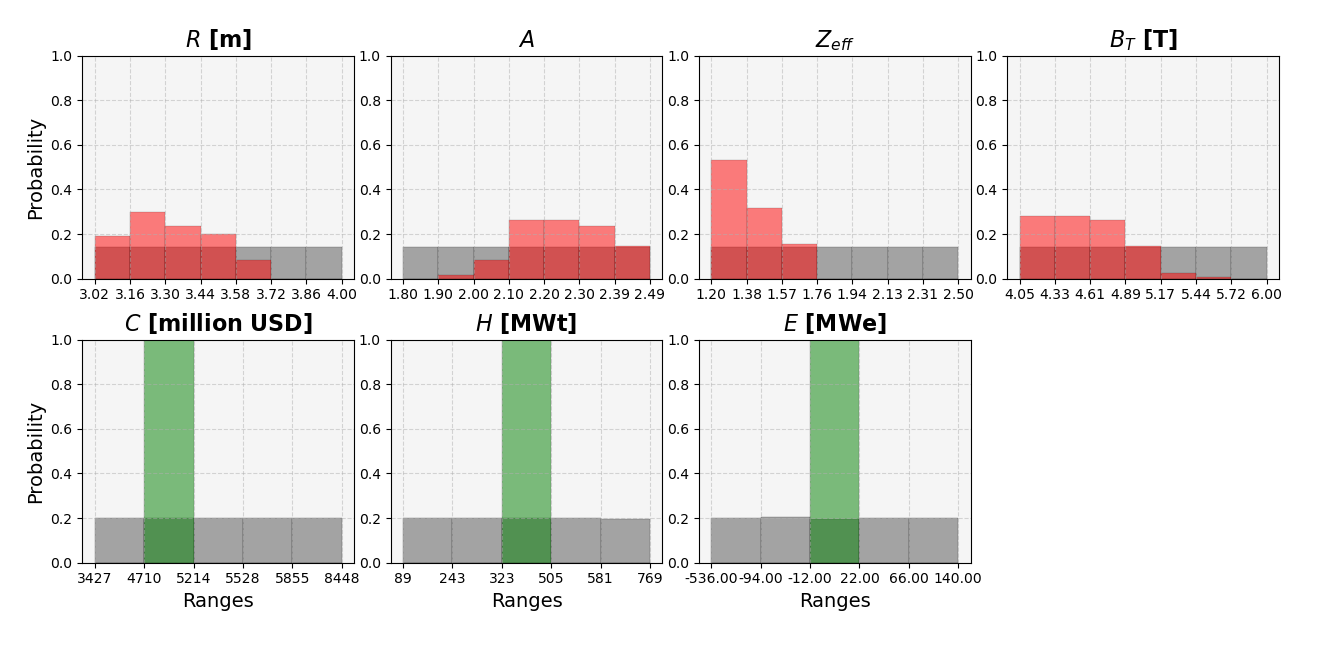
\includegraphics[width=0.6\textwidth]{figures/TE_results/march_data/config(57)_3outputs_V2_2.png}
    \caption{Resulting posterior distributions depicted in red (variables: Major Radius $R$, Aspect Ratio $A$, Effective Ion Charge $Z_{\text{eff}}$, Toroidal Field on Plasma $B_{\text{T}}$) for reverse
    inference on the selected green bins (High Grade Wasteheat $H$, Net Electrical Output $E$, and  Capital Cost $C$) after updating the marginal prior beliefs (grey).}~\label{fig:config(57)_3outputs_V2_2}
\end{figure*}

\begin{figure*}[ht]
    \centering
    \includegraphics[width=0.6\textwidth]{figures/TE_results/march_data/config(57)_3outputs_V2_3.png}
    \caption{Resulting posterior distributions depicted in red (variables: Major Radius $R$, Aspect Ratio $A$, Effective Ion Charge $Z_{\text{eff}}$, Toroidal Field on Plasma $B_{\text{T}}$) for reverse
    inference on the selected green bins (High Grade Wasteheat $H$, Net Electrical Output $E$, and  Capital Cost $C$) after updating the marginal prior beliefs (grey).}~\label{fig:config(57)_3outputs_V2_3}
\end{figure*}


\begin{figure*}[ht]
    \centering
    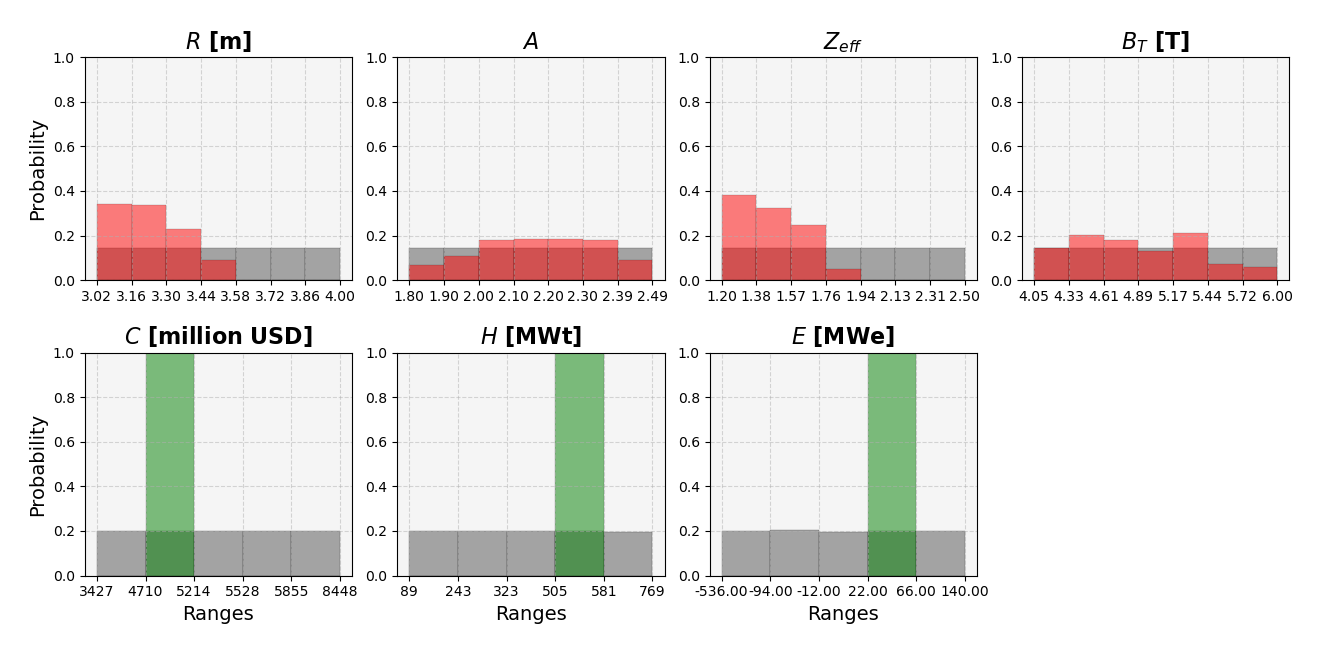
\includegraphics[width=0.6\textwidth]{figures/TE_results/march_data/config(57)_3outputs_v2_5.png}
    \caption{Resulting posterior distributions depicted in red (variables: Major Radius $R$, Aspect Ratio $A$, Effective Ion Charge $Z_{\text{eff}}$, Toroidal Field on Plasma $B_{\text{T}}$) for reverse
    inference on the selected green bins (High Grade Wasteheat $H$, Net Electrical Output $E$, and  Capital Cost $C$) after updating the marginal prior beliefs (grey).}~\label{fig:config(57)_3outputs_V2_5}
\end{figure*}

\begin{figure*}[ht]
    \centering
    \includegraphics[width=0.6\textwidth]{figures/TE_results/march_data/config(57)_3outputs_V2_6.png}
    \caption{Resulting posterior distributions depicted in red (variables: Major Radius $R$, Aspect Ratio $A$, Effective Ion Charge $Z_{\text{eff}}$, Toroidal Field on Plasma $B_{\text{T}}$) for reverse
    inference on the selected green bins (High Grade Wasteheat $H$, Net Electrical Output $E$, and  Capital Cost $C$) after updating the marginal prior beliefs (grey).}~\label{fig:config(57)_3outputs_V2_6}
\end{figure*}

\begin{figure*}[ht]
    \centering
    \includegraphics[width=0.6\textwidth]{figures/TE_results/march_data/config(57)_3outputs_V2_7.png}
    \caption{Resulting posterior distributions depicted in red (variables: Major Radius $R$, Aspect Ratio $A$, Effective Ion Charge $Z_{\text{eff}}$, Toroidal Field on Plasma $B_{\text{T}}$) for reverse
    inference on the selected green bins (High Grade Wasteheat $H$, Net Electrical Output $E$, and  Capital Cost $C$) after updating the marginal prior beliefs (grey).}~\label{fig:config(57)_3outputs_V2_7}
\end{figure*}

\begin{figure*}[ht]
    \centering
    \includegraphics[width=0.6\textwidth]{figures/TE_results/march_data/config(57)_3outputs_V2_8.png}
    \caption{Resulting posterior distributions depicted in red (variables: Major Radius $R$, Aspect Ratio $A$, Effective Ion Charge $Z_{\text{eff}}$, Toroidal Field on Plasma $B_{\text{T}}$) for reverse
    inference on the selected green bins (High Grade Wasteheat $H$, Net Electrical Output $E$, and  Capital Cost $C$) after updating the marginal prior beliefs (grey).}~\label{fig:config(57)_3outputs_V2_8}
\end{figure*}

\begin{figure*}[ht]
    \centering
    \includegraphics[width=0.6\textwidth]{figures/TE_results/march_data/config(57)_3outputs_V2_9.png}
    \caption{Resulting posterior distributions depicted in red (variables: Major Radius $R$, Aspect Ratio $A$, Effective Ion Charge $Z_{\text{eff}}$, Toroidal Field on Plasma $B_{\text{T}}$) for reverse
    inference on the selected green bins (High Grade Wasteheat $H$, Net Electrical Output $E$, and  Capital Major Radius $R$Cost $C$) after updating the marginal prior beliefs (grey).}~\label{fig:config(57)_3outputs_V2_9}
\end{figure*}

\begin{figure*}[ht]
    \centering
    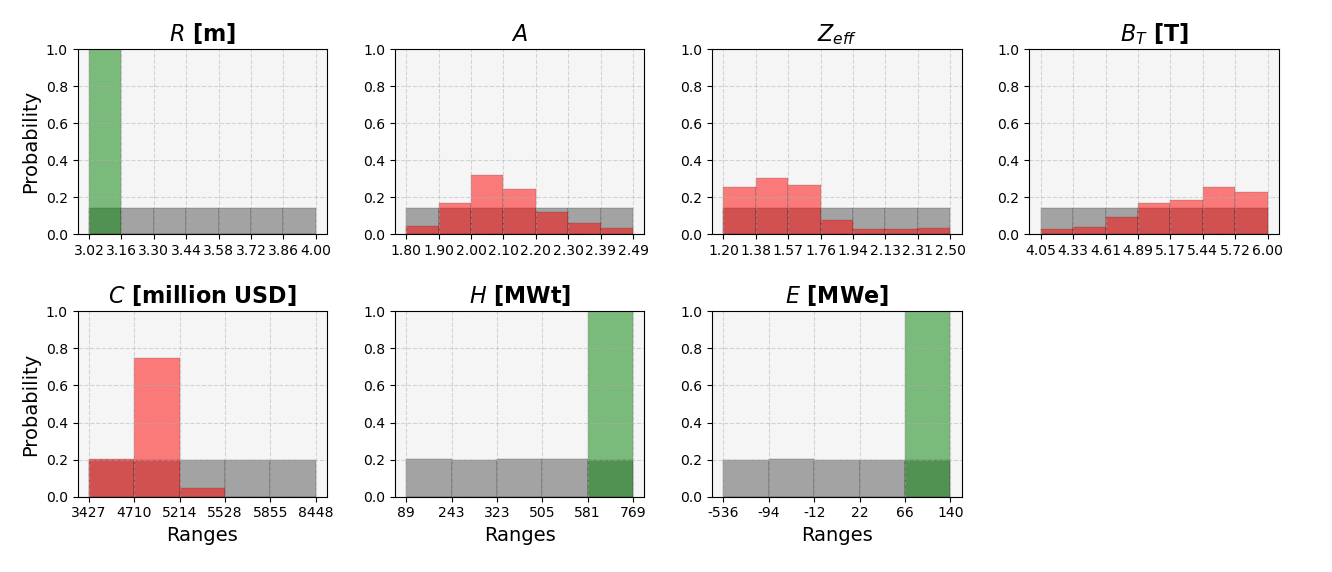
\includegraphics[width=0.6\textwidth]{figures/TE_results/march_data/config(57)_outputs(3)_hybrid_2.png}
    \caption{Resulting posterior distributions depicted in red (variables: Aspect Ratio $A$, Effective Ion Charge $Z_{\text{eff}}$, Toroidal Field on Plasma $B_{\text{T}}$ and Capital Cost $C$) for hybrid
    inference on the selected green bins (High Grade Wasteheat $H$, Net Electrical Output $E$, and Major Radius $R$) after updating the marginal prior beliefs (grey).}~\label{fig:config(57)_outputs(3)_hybrid_2}
\end{figure*}

\begin{figure*}[ht]
    \centering
    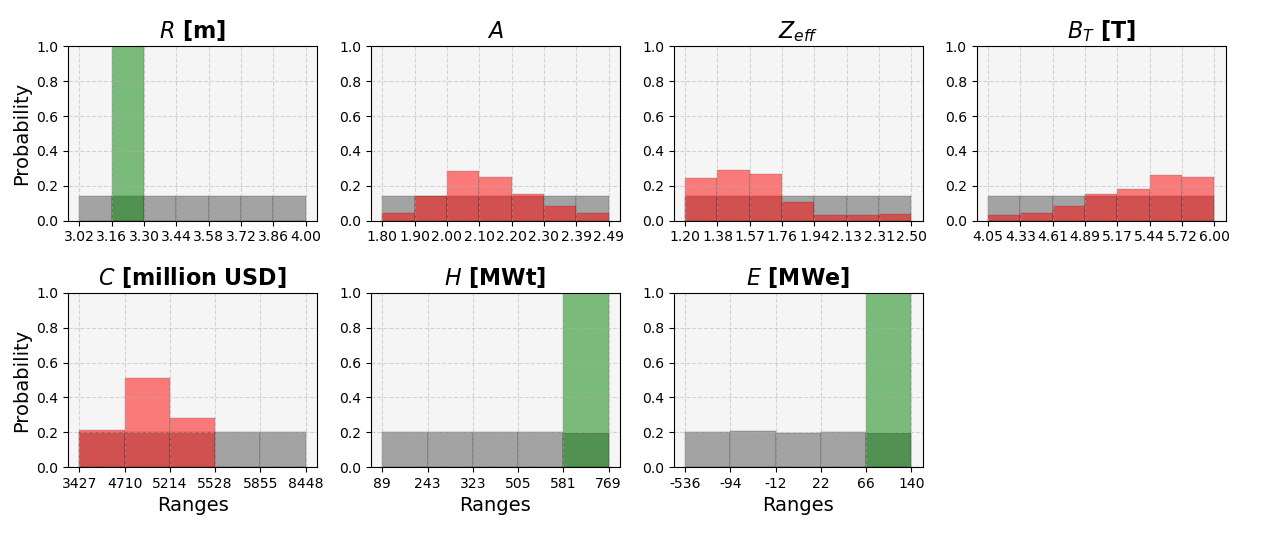
\includegraphics[width=0.6\textwidth]{figures/TE_results/march_data/config(57)_outputs(3)_hybrid_3.png}
    \caption{Resulting posterior distributions depicted in red (variables: Aspect Ratio $A$, Effective Ion Charge $Z_{\text{eff}}$, Toroidal Field on Plasma $B_{\text{T}}$ and Capital Cost $C$) for hybrid
    inference on the selected green bins (High Grade Wasteheat $H$, Net Electrical Output $E$, and Major Radius $R$) after updating the marginal prior beliefs (grey).}~\label{fig:config(57)_outputs(3)_hybrid_3}
\end{figure*}

\begin{figure*}[ht]
    \centering
    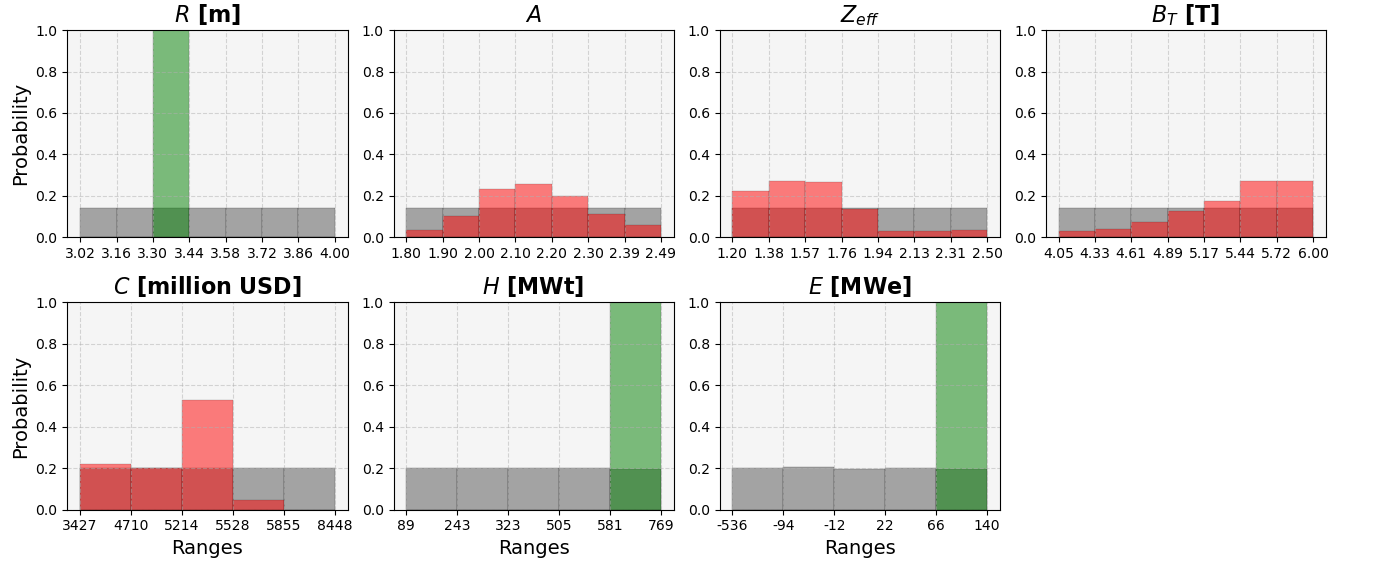
\includegraphics[width=0.6\textwidth]{figures/TE_results/march_data/config(57)_outputs(3)_hybrid4.png}
    \caption{Resulting posterior distributions depicted in red (variables: Aspect Ratio $A$, Effective Ion Charge $Z_{\text{eff}}$, Toroidal Field on Plasma $B_{\text{T}}$ and Capital Cost $C$) for hybrid
    inference on the selected green bins (High Grade Wasteheat $H$, Net Electrical Output $E$, and Major Radius $R$) after updating the marginal prior beliefs (grey).}~\label{fig:config(57)_outputs(3)_hybrid4}
\end{figure*}

\begin{figure*}[ht]
    \centering
    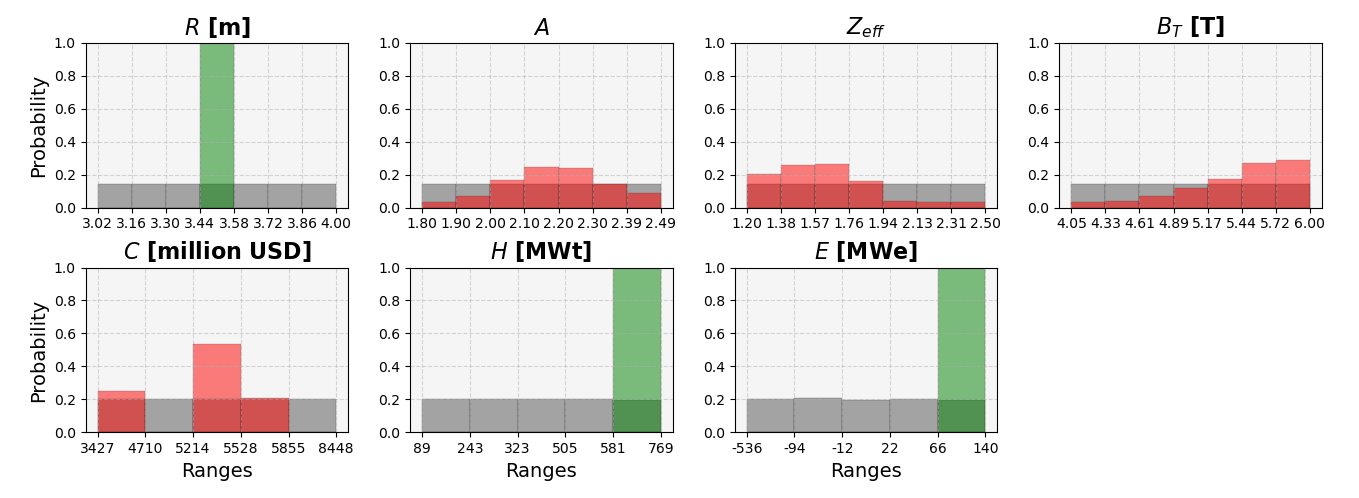
\includegraphics[width=0.6\textwidth]{figures/TE_results/march_data/config(57)_outputs(3)_hybrid5.png}
    \caption{Resulting posterior distributions depicted in red (variables: Aspect Ratio $A$, Effective Ion Charge $Z_{\text{eff}}$, Toroidal Field on Plasma $B_{\text{T}}$ and Capital Cost $C$) for hybrid
    inference on the selected green bins (High Grade Wasteheat $H$, Net Electrical Output $E$, and Major Radius $R$) after updating the marginal prior beliefs (grey).}~\label{fig:config(57)_outputs(3)_hybrid5}
\end{figure*}

\begin{figure*}[ht]
    \centering
    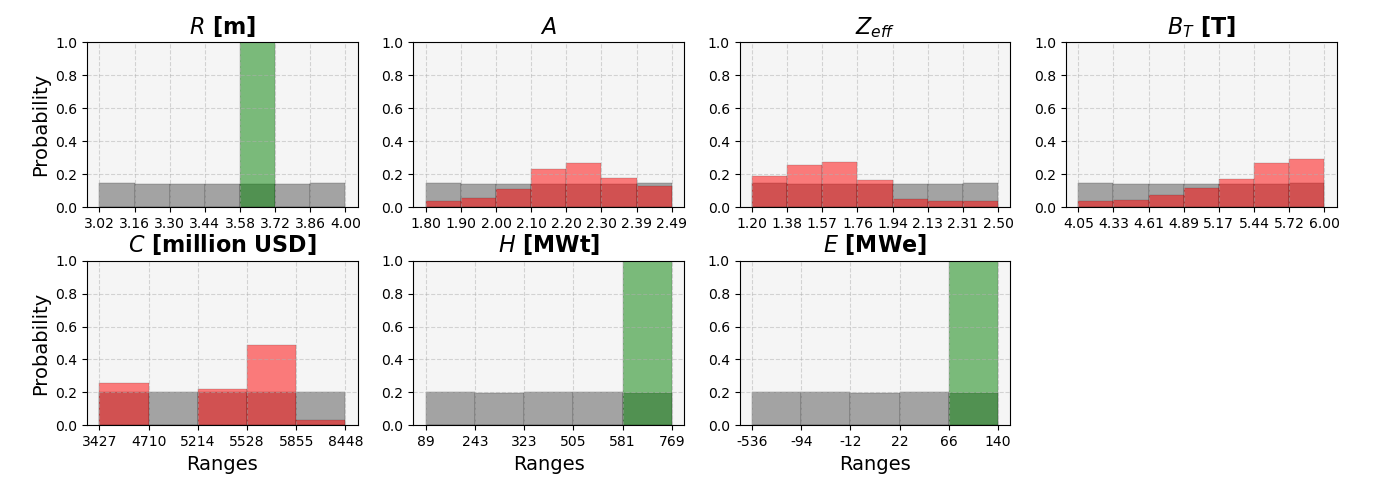
\includegraphics[width=0.6\textwidth]{figures/TE_results/march_data/config(57)_outputs(3)_hybrid6.png}
    \caption{Resulting posterior distributions depicted in red (variables: Aspect Ratio $A$, Effective Ion Charge $Z_{\text{eff}}$, Toroidal Field on Plasma $B_{\text{T}}$ and Capital Cost $C$) for hybrid
    inference on the selected green bins (High Grade Wasteheat $H$, Net Electrical Output $E$, and Major Radius $R$) after updating the marginal prior beliefs (grey).}~\label{fig:config(57)_outputs(3)_hybrid6}
\end{figure*}

\begin{figure*}[ht]
    \centering
    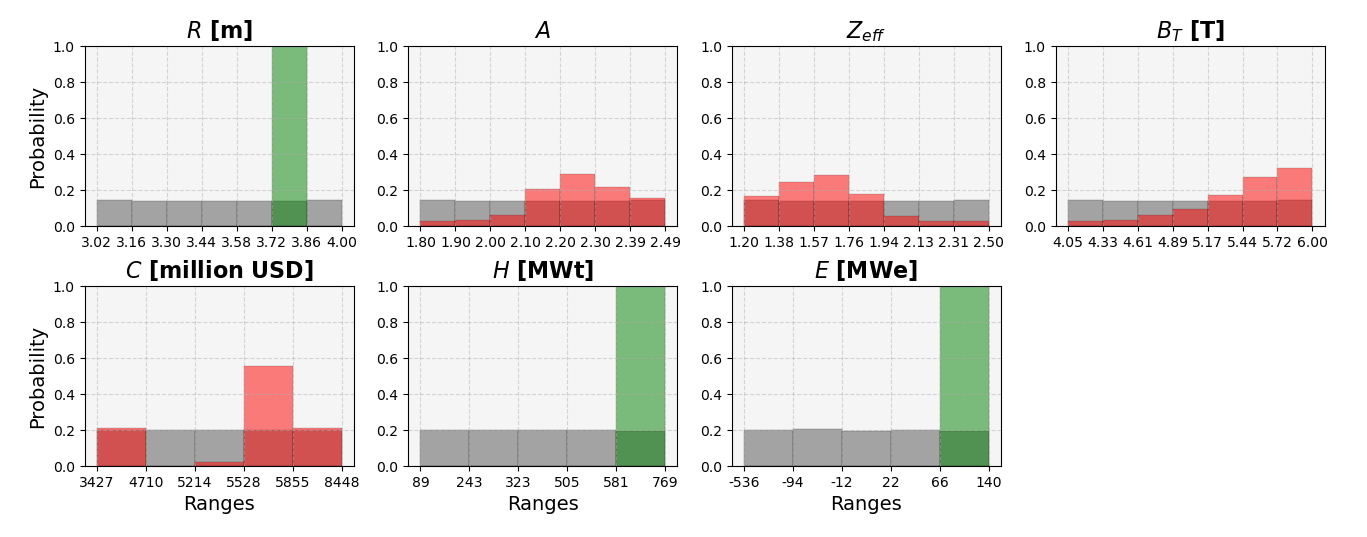
\includegraphics[width=0.6\textwidth]{figures/TE_results/march_data/config(57)_outputs(3)_hybrid7.png}
    \caption{Resulting posterior distributions depicted in red (variables: Aspect Ratio $A$, Effective Ion Charge $Z_{\text{eff}}$, Toroidal Field on Plasma $B_{\text{T}}$ and Capital Cost $C$) for hybrid
    inference on the selected green bins (High Grade Wasteheat $H$, Net Electrical Output $E$, and Major Radius $R$) after updating the marginal prior beliefs (grey).}~\label{fig:config(57)_outputs(3)_hybrid7}
\end{figure*}


\begin{figure*}[ht]
    \centering
    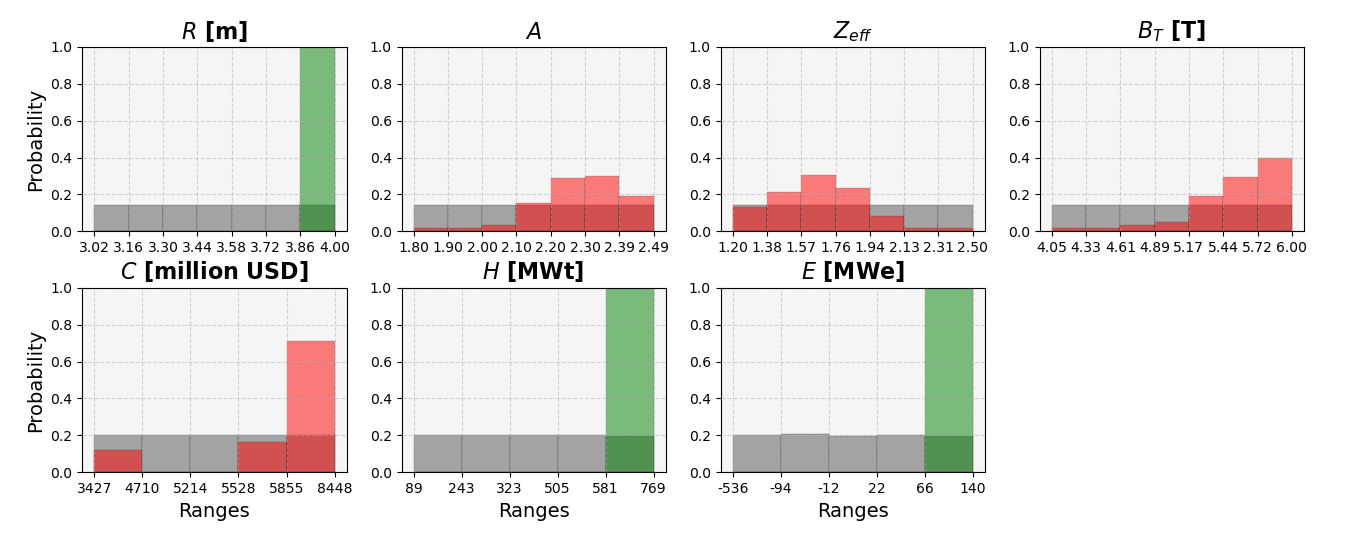
\includegraphics[width=0.6\textwidth]{figures/TE_results/march_data/config(57)_outputs(3)_hybrid8.png}
    \caption{Resulting posterior distributions depicted in red (variables: Aspect Ratio $A$, Effective Ion Charge $Z_{\text{eff}}$, Toroidal Field on Plasma $B_{\text{T}}$ and Capital Cost $C$) for hybrid
    inference on the selected green bins (High Grade Wasteheat $H$, Net Electrical Output $E$, and Major Radius $R$) after updating the marginal prior beliefs (grey).}~\label{fig:config(57)_outputs(3)_hybrid8}
\end{figure*}

% 4 outputs: 

% \begin{figure*}[ht]
%     \centering
%     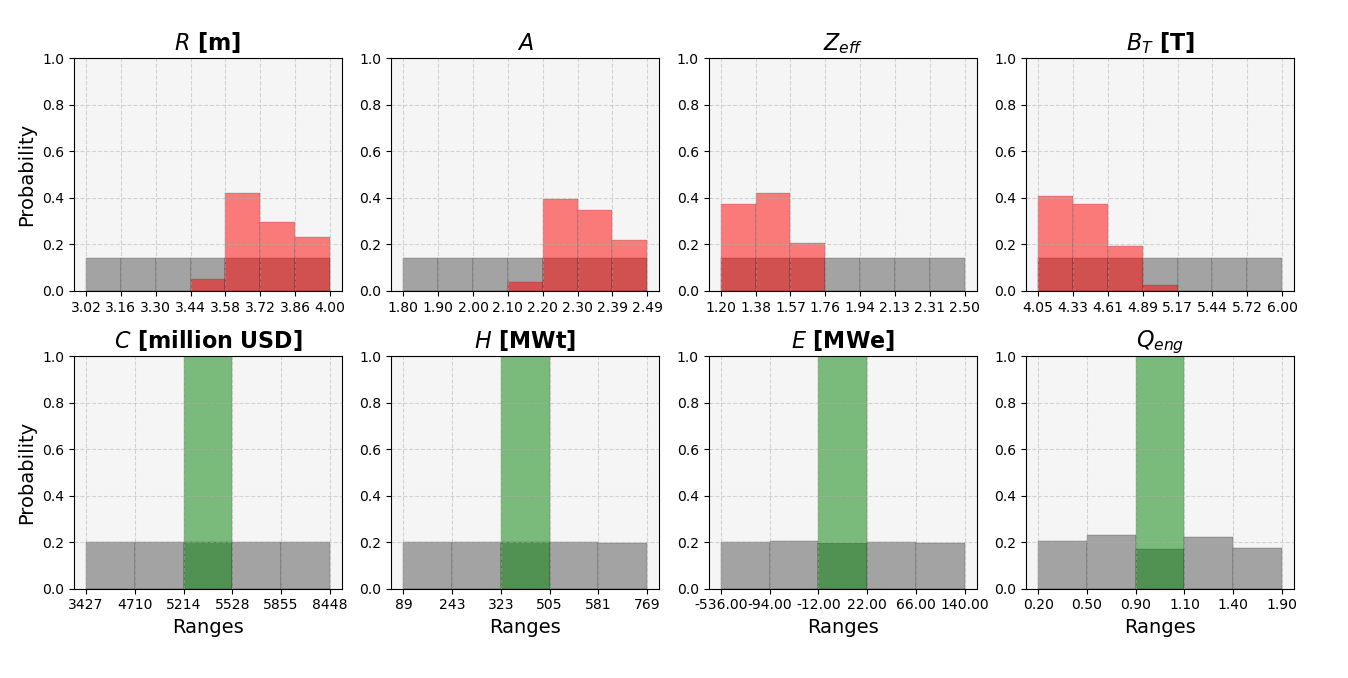
\includegraphics[width=0.6\textwidth]{figures/TE_results/march_data/config(57)_4outputs_1.png}
%     \caption{Resulting posterior distributions depicted in red (variables: Major Radius $R$, Aspect Ratio $A$, Effective Ion Charge $Z_{\text{eff}}$, Toroidal Field on Plasma $B_{\text{T}}$) for reverse
%     inference on the selected green bins (High Grade Wasteheat $H$, Net Electrical Output $E$, Capital Cost $C$, and Engineering Quality $Q_{\text{eng}}$) after updating the marginal prior beliefs (grey).}~\label{fig:config(57)_4outputs_1}
% \end{figure*}

% \begin{figure*}[ht]
%     \centering
%     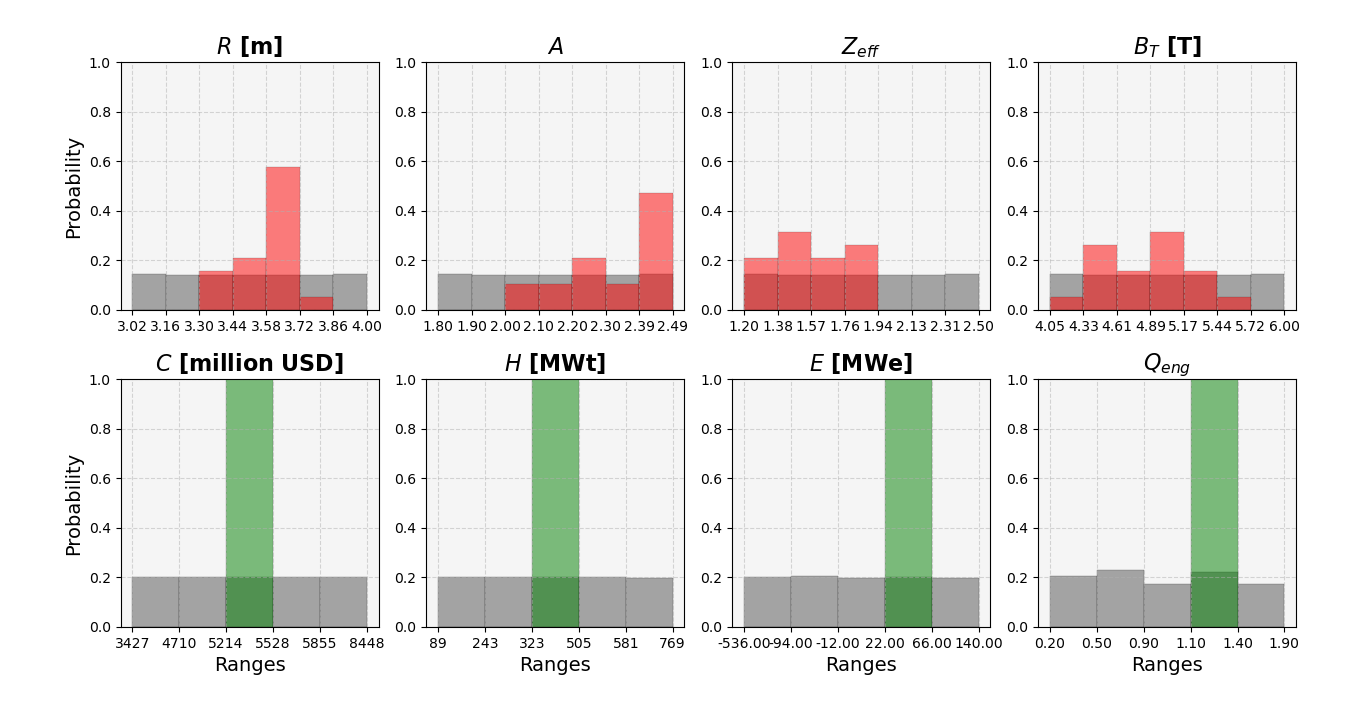
\includegraphics[width=0.6\textwidth]{figures/TE_results/march_data/config(57)_outputs(4)8.png}
%     \caption{Resulting posterior distributions depicted in red (variables: Major Radius $R$, Aspect Ratio $A$, Effective Ion Charge $Z_{\text{eff}}$, Toroidal Field on Plasma $B_{\text{T}}$) for reverse
%     inference on the selected green bins (High Grade Wasteheat $H$, Net Electrical Output $E$, Capital Cost $C$, and Engineering Quality $Q_{\text{eng}}$) after updating the marginal prior beliefs (grey).}~\label{fig:config(57)_outputs(4)8}
% \end{figure*}

% \begin{figure*}[ht]
%     \centering
%     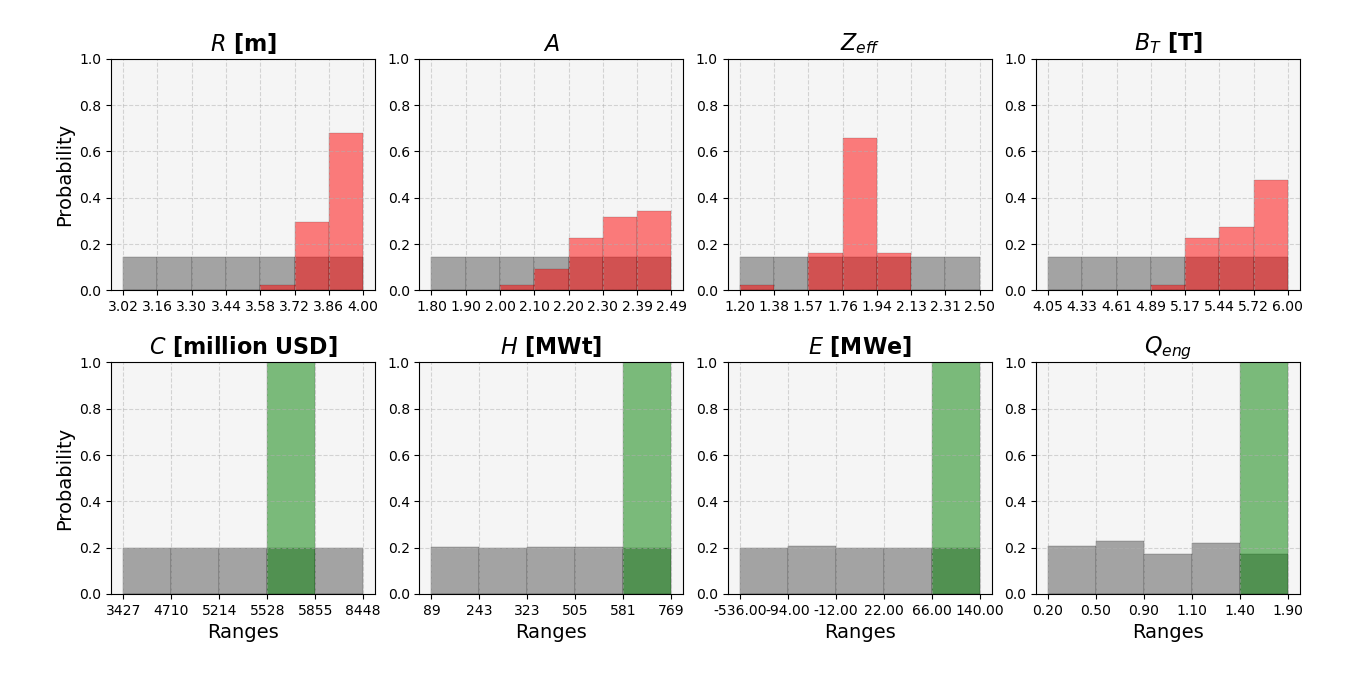
\includegraphics[width=0.6\textwidth]{figures/TE_results/march_data/config(57)_outputs(4)3.png}
%     \caption{Resulting posterior distributions depicted in red (variables: Major Radius $R$, Aspect Ratio $A$, Effective Ion Charge $Z_{\text{eff}}$, Toroidal Field on Plasma $B_{\text{T}}$) for reverse
%     inference on the selected green bins (High Grade Wasteheat $H$, Net Electrical Output $E$, Capital Cost $C$, and Engineering Quality $Q_{\text{eng}}$) after updating the marginal prior beliefs (grey).}~\label{fig:config(57)_outputs(4)3}
% \end{figure*}

% \begin{figure*}[ht]
%     \centering
%     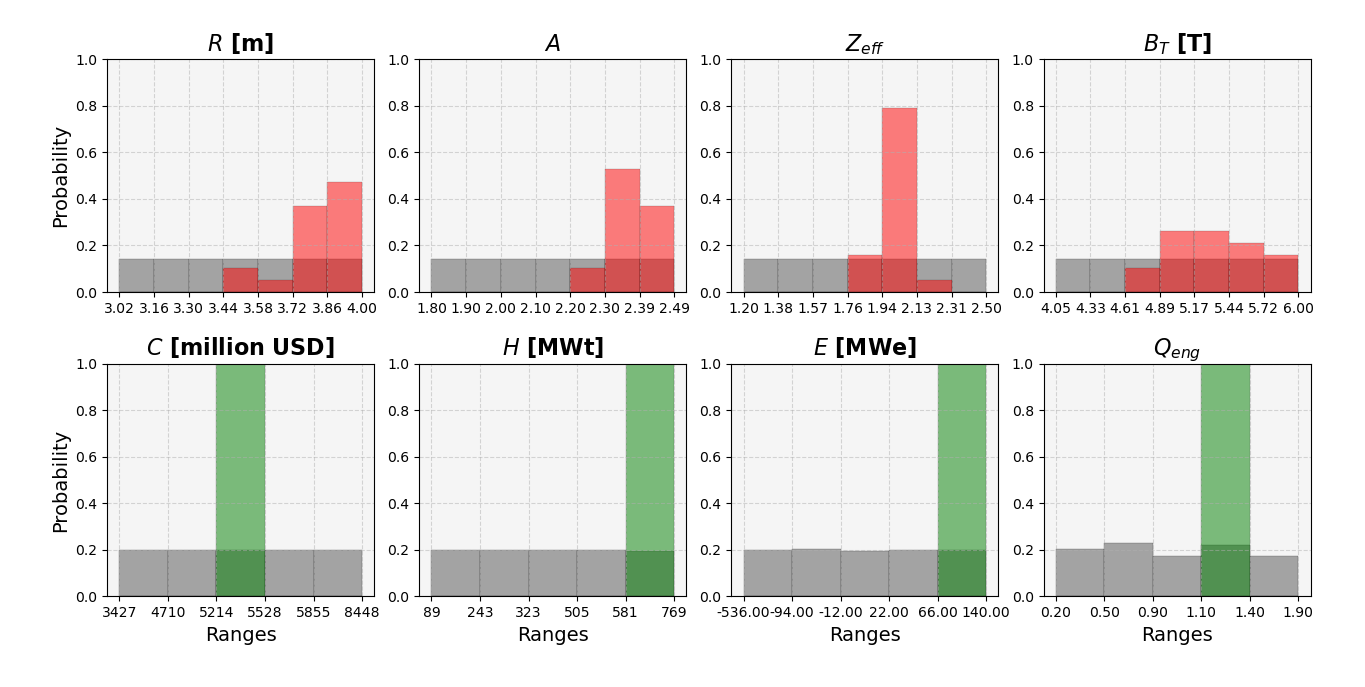
\includegraphics[width=0.6\textwidth]{figures/TE_results/march_data/config(57)_outputs(4)5.png}
%     \caption{Resulting posterior distributions depicted in red (variables: Major Radius $R$, Aspect Ratio $A$, Effective Ion Charge $Z_{\text{eff}}$, Toroidal Field on Plasma $B_{\text{T}}$) for reverse
%     inference on the selected green bins (High Grade Wasteheat $H$, Net Electrical Output $E$, Capital Cost $C$, and Engineering Quality $Q_{\text{eng}}$) after updating the marginal prior beliefs (grey).}~\label{fig:config(57)_outputs(4)5}
% \end{figure*}

% \begin{figure*}[ht]
%     \centering
%     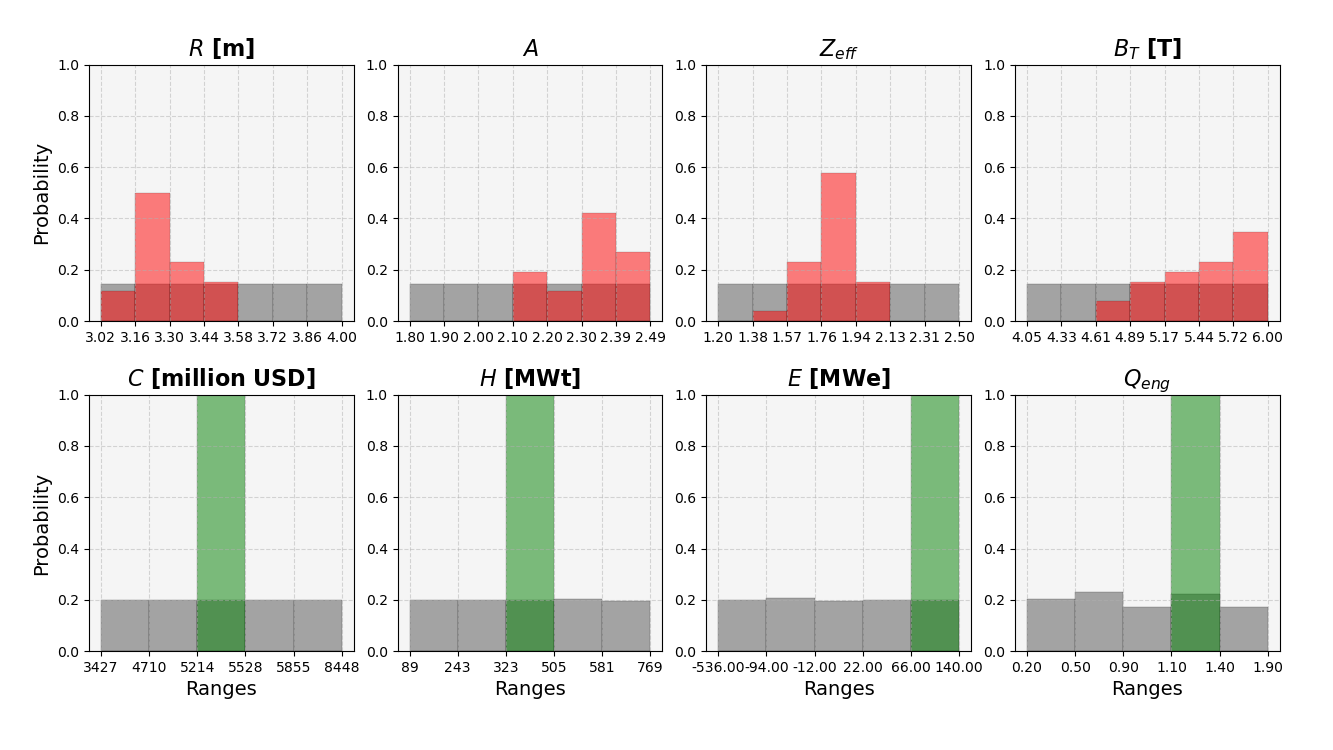
\includegraphics[width=0.6\textwidth]{figures/TE_results/march_data/config(57)_outputs(4)9.png}
%     \caption{Resulting posterior distributions depicted in red (variables: Major Radius $R$, Aspect Ratio $A$, Effective Ion Charge $Z_{\text{eff}}$, Toroidal Field on Plasma $B_{\text{T}}$) for reverse
%     inference on the selected green bins (High Grade Wasteheat $H$, Net Electrical Output $E$, Capital Cost $C$, and Engineering Quality $Q_{\text{eng}}$) after updating the marginal prior beliefs (grey).}~\label{fig:config(57)_outputs(4)9}
% \end{figure*}